%-----先用xelatex编译，再用lualatex编译------

\documentclass[12pt,a4paper]{article}
\usepackage[UTF8]{ctex}
\usepackage{amsmath, amssymb, amsthm}
\usepackage{geometry}
\usepackage{enumitem}
\usepackage{fancyhdr}
\usepackage{titlesec}
\usepackage{xcolor}
\usepackage{fontspec}
\usepackage{graphicx}



%===========强制加粗，需用lualatex编译，在字体设置后加以下内容，若无需加粗可去掉=============

%		[
%	FakeBold=1.5,
%	AutoFakeBold=true
%	]



% ========== 中文字体，强制加粗====================

\setCJKmainfont{SimSun}[
BoldFont={SimHei},
FakeBold=1.5,
AutoFakeBold=true
]
\setCJKsansfont{SimHei}[
BoldFont={SimHei},
FakeBold=1.5,
AutoFakeBold=true
]
\setCJKfamilyfont{kai}{KaiTi}[
FakeBold=1.5,
AutoFakeBold=true
]
\setCJKfamilyfont{hei}{SimHei}[
FakeBold=1.5,
AutoFakeBold=true
]
\newcommand{\kai}{\CJKfamily{kai}}
\newcommand{\hei}{\CJKfamily{hei}}




% ========== 英文字体，强制加粗 ==========
% 数学模式使用 Times 风格
\usepackage{unicode-math}
\setmainfont{Times New Roman}[
FakeBold=1.5,
AutoFakeBold=true
]
\setmathfont{TeX Gyre Termes Math}[
FakeBold=1.5,
AutoFakeBold=true
]  % Times 风格的数学字体



% ========== 页面设置 ==========
\geometry{left=2cm, right=2cm, top=2.5cm, bottom=2.5cm}

% ========== 页眉页脚 ==========
\pagestyle{fancy}
\fancyhf{}
\cfoot{\small 高三数学 第\thepage 页（共4页）}
\renewcommand{\headrulewidth}{0pt}
\renewcommand{\footrulewidth}{0pt}



% ========== 选项环境 ==========
%1.选项较短用\choice{A}{B}{C}{D}
\newcommand{\choices}[4]{%
	\par\noindent
	\begin{tabular}{@{}p{0.22\linewidth}p{0.22\linewidth}p{0.22\linewidth}p{0.22\linewidth}@{}}
		A. #1 & B. #2 & C. #3 & D. #4
	\end{tabular}%
	\par
}

%2.选项较长用\Choice{A}{B}{C}{D}
\newcommand{\Choices}[4]{%
	\par\noindent
	\begin{tabular}{@{}p{0.44\linewidth}p{0.44\linewidth}@{}}
		A. #1 & B. #2
	\end{tabular}%
	\par
	\par\noindent
	\begin{tabular}{@{}p{0.44\linewidth}p{0.44\linewidth}@{}}
		C. #3 & D. #4
	\end{tabular}%
	\par
}


% ========== 列表间距 ==========
\setlist[enumerate,1]{label=\arabic*., left=0pt, itemsep=12pt, parsep=0pt, topsep=0pt}
\setlist[enumerate,2]{left=0pt, itemsep=2pt, labelsep=0.5em}

%enumerate 是 LaTeX 中用于创建自动编号列表的环境，可嵌套
%	\begin{enumerate}
%		\item 第一项
%		\item 第二项
%		\item 第三项
%	\end{enumerate}


%================================开始=======================================
\begin{document}

% ========== 第1页，需手动用\newpage 分页！==================
	% ========== 标题部分 ==========
	\begin{center}
		{\LARGE 清苑一中2026届高一年级六月供题}

		\vspace{1cm}
		{\hei\huge 数 \quad 学}
	\end{center}

	\vspace{0.3cm}

	% 双横线 + 左右两侧文字（楷体）
	\noindent
	\begin{minipage}[b]{0.5\textwidth}
		\raggedright
		{\kai 清苑一中高一数学组命制}
	\end{minipage}%
	\begin{minipage}[b]{0.5\textwidth}
		\raggedleft
		{\kai 2026.6}
	\end{minipage}
	\\[-11pt]
	\noindent\rule{\textwidth}{1pt}\\[-16pt]
	\noindent\rule{\textwidth}{1pt}
	\\[-20pt]

	% ========== 试卷说明 ==========
	{\hei\noindent\hspace{2em}本卷共4页，19题，全卷满分150分。用时120分钟。}

	\vspace{0.5cm}

	% ========== 注意事项 ==========
	{\hei\noindent 注意事项：}
	\begin{enumerate}[left=2em, itemsep=2pt, labelsep=0.5em, topsep=0pt]
		\item {\kai 选择题的作答：每小题选出答案后，用2B铅笔把答题卡上对应题目的答案标号涂黑。}
		\item {\kai 非选择题的作答：用黑色签字笔直接答在答题卡上对应的答题区域内。}
	\end{enumerate}

	\vspace{0.3cm}

	% ========== 单选 =========
	{\hei\noindent 一、单项选择题：本题共8小题，每小题5分，共40分。在每小题给出的四个选项中，只有一项是符合题目要求。}

	\vspace{0.3cm}

	\begin{enumerate}

		\item 已知 \( f(\tan x) = \sin 2x + \cos^2 x \)，则 \( f(\cos \frac{5\pi}{3}) = \)
		\choices{\(\dfrac{8}{5}\)}{\(0\)}{\(\dfrac{4\sqrt{3} + 4}{7}\)}{\(\dfrac{4 - 4\sqrt{3}}{7}\)}


		\item 对函数 \( y = x^2 \) 和 \( y = \tan x \) 的图象与性质，有下面四个结论：
		\begin{enumerate}
				\item[\textcircled{1}] 它们的定义域不同，但值域相同；
				\item[\textcircled{2}] 它们在各自的定义域内都是增函数；
				\item[\textcircled{3}] 它们在各自的定义域内都是奇函数；
				\item[\textcircled{4}]  它们中一个是周期函数，另一个不是周期函数
		\end{enumerate}
			其中所有正确结论的编号是
		\choices{"\textcircled{1}\textcircled{2} \textcircled{3}  "}{\textcircled{1} \textcircled{2} \textcircled{4} }{\textcircled{1} \textcircled{3} \textcircled{4} }{\textcircled{2} \textcircled{3} \textcircled{4} }


		\item 已知函数 \( y = f(x) \) 的定义域为 \([-8,1]\)，则函数 \( g(x) = \dfrac{f(2x+1)}{x+2} \) 的定义域是
		\choices{\((-\infty, -2) \cup (2, 3]\)}{\((-8, -2) \cup (-2, 1]\)}{\([-2, -8) \cup (1, 2]\)}{\([-2, 0) \cup (2, 3]\)}

		\item 已知 \( a = \log_{0.2} 0.3 \)，\( b = \log_{0.3} 0.2 \)，\( c = \log_{2} 3 \)，则 \( a, b, c \) 的大小关系为
		\choices{\(b < c < a\)}{\(c < b < a\)}{\(a < b < c\)}{\(a < c < b\)}

		\item 已知集合 \( A = \{y \mid y = x^2 + 2x - 2\} \)，\( B = \{y \mid y = -x^2 + 2x + 6\} \)，则 \( A \cap B = \)
		\choices{\((-2, -2)\)}{\((-2, 2)\)}{\((-2, -6)\)}{\((-2, 6)\)}

		\item 设 \( f(x) = \sin(\alpha x + \beta) \)，若 \( \sin \alpha = 3 \sin(\alpha + 2\beta) \)，则 \( \alpha = \)
		\choices{\(\dfrac{\sqrt{2}}{4}\)}{\(\dfrac{\sqrt{2}}{4}\)}{\(\dfrac{\sqrt{2}}{2}\)}{\(\dfrac{\sqrt{2}}{2}\)}



		\item 设函数 \( f(x) = 2\sin\left(\omega x - \dfrac{\pi}{6}\right) - 	1(\omega > 0) \) 在 \( [\pi, 2\pi] \) 上至少有两个不同零点，则实数 \( \omega \) 的取值范围是
		\Choices{\(\left( \dfrac{3}{2}, +\infty \right)\)}{\(\left( \dfrac{3}{2}, \dfrac{7}{3} \right] \cup \left( \dfrac{5}{2}, +\infty \right)\)}{\(\left( \dfrac{13}{6}, 3 \right] \cup \left( \dfrac{19}{6}, +\infty \right)\)}{\(\left( \dfrac{1}{2}, +\infty \right)\)}



		\item 已知 \( \alpha, \beta \in \left( 0, \dfrac{\pi}{2} \right) \)，\( 2\sin\beta = \cos(\alpha + \beta)\sin\alpha \)，则 \( \tan\beta \) 的最大值为
		\choices{\(\dfrac{\sqrt{6}}{12}\)}{\(\dfrac{\sqrt{6}}{6}\)}{\(\dfrac{\sqrt{6}}{4}\)}{\(\dfrac{\sqrt{3}}{6}\)}

	\end{enumerate}






	%============多选==============
	{\hei\noindent 二、多项选择题：本题共3小题，每小题6分，共18分。在每小题给出的选项中，有多项符合题目要求。全部选对的得6分，部分选对的得部分分，有选错的得0分。}

	\vspace{0.3cm}

	\begin{enumerate}[resume]	%[resume] 是 enumitem 宏包提供的一个选项，用于让编号从上一次结束的地方继续。


		\item 已知 \( \omega > 0 \)，函数 \( f(x) = \sin \omega x \cos \omega x + \sqrt{3} \cos^2 \omega x - \dfrac{\sqrt{3}}{2} \) 的最小正周期为 \( 2\pi \)，则下列结论正确的是
		\Choices{\(\omega = 1\)}{函数 \( f(x) \) 在区间 \( \left[ -\dfrac{\pi}{12}, \dfrac{\pi}{12} \right] \) 上单调递增}{将函数 \( f(x) \) 的图象向左平移 \( \dfrac{\pi}{6} \) 个单位长度可得函数 \( g(x) = \cos x \) 的图象}{函数 \( f(x) \) 的图象关于直线 \( x = \dfrac{\pi}{2} \) 对称}

		\item 已知函数 \( f(x) = \sqrt{3} \sin 2\omega x + \cos 2\omega x (\omega > 0) \) 的零点构成一个公差为 \( \dfrac{\pi}{2} \) 的等差数列，把 \( f(x) \) 的图象沿 \( x \) 轴向右平移 \( \dfrac{\pi}{3} \) 个单位长度得到函数 \( g(x) \) 的图象，则
		\Choices{\(g(x)\) 在 \( \left[ \dfrac{\pi}{4}, \dfrac{\pi}{2} \right] \) 上单调递增}{\(g(x)\) 在区间 \( \left[ \dfrac{\pi}{6}, \dfrac{\pi}{3} \right] \) 上的值域为 \( [0, 2] \)}{\(g(x)\) 是奇函数}{\(g(x)\) 在区间 \( \left[ \dfrac{\pi}{6}, \dfrac{\pi}{3} \right] \) 上的值域为 \( [0, 2] \)}

		\item \( f(x) \) 是定义在 \( \mathbb{R} \) 上的奇函数，满足 \( f(1-x) = f(3+x) \) 且 \( f(x) \) 在 \( [0, 2] \) 上为单调递减的一次函数，\( f(1) = -1 \)，则
		\Choices{函数 \( f(x) \) 图象关于直线 \( x = 2 \) 对称}{函数 \( f(x) \) 的最小正周期为 \( 6 \)}{\( f(2026) + f(2025) = -3 \)}{设 \( g(x) = e^{x+2} (-6 < x < 2) \)，\( f(x) \) 和 \( g(x) \) 的图象所有交点横坐标之和为 \( -4 \)}
	\end{enumerate}

	\vspace{0.5cm}



	%===================填空=======================================
	{\hei\noindent 三、填空题：本题共3小题，每小题5分，共15分。}

	\vspace{0.3cm}

	\begin{enumerate}[resume]


	\item \( \sin 50^\circ \left( \dfrac{1}{8} + \sqrt{3} \tan 10^\circ \right) = \) \underline{\hspace{2cm}}.

	\item 已知集合 \( A = \{x \in \mathbb{R} \mid p x = 10, p \in \mathbb{N}\} \)，\( B = \{x \in \mathbb{R} \mid x > a\} \)，若 \( A \cup B = B \)，则实数 \( a \) 的取值范围是 \underline{\hspace{2cm}}.

	\item 设函数 \( f(x) \) 的定义域为 \( \mathbb{R} \)，且 \( f(x+1) \) 为偶函数，\( f(x-1) \) 为奇函数，当 \( x \in [-1, 1] \) 时，$ f(x)=1-x^2,\quad f(1)+f(2)+f(3)+\cdots+f(2025) =$  \underline{\hspace{2cm}}.

	\end{enumerate}

	\vspace{0.5cm}


	%=========================大题===========================================
	{\hei\noindent 四、解答题：本题共5小题，共77分。解答应写出文字说明、证明过程或演算步骤。}

	\vspace{0.3cm}

	\begin{enumerate}[resume]



		\item （13分）
		计算：
		\begin{enumerate}
			\item[(1)] $\quad \left( \frac{16}{81} \right)^{\frac{1}{4}} - \sqrt{4^{\frac{1}{3}} \times 2^{\frac{1}{2}}} + \left( \sqrt{5} - 2 \right)^0.$
			\item[(2)] $ \quad \lg 2 + \lg \frac{5}{8} - \lg \frac{25}{2} + \log_4 9 \cdot \log_9 8.$
		\end{enumerate}



		\vspace{0.5cm}

		\item （15分）

		我国核电建设占全球在建核电机组的 \(40\%\) 以上，是全球核电在建规模最大的国家。核电抗飞溅结构是保障核电工程安全的重要基础设施，为此国家制定了一系列核电钢筋混凝土施工细则，连接技术全面采用 HRB500 高强钢筋替代 HRB400 及以下钢筋。某项目课题组针对 HRB500 高强钢筋的现场加工难题，对螺纹滚道几何成形机理进行了深入研究，研究发现某 S 型螺纹丝杠旋绕的滚道径向残留高度 \( y \)（单位：mm）关于滚道径向方位角 \( x \)（单位：rad）的函数 \( y = f(x) \) 近似地满足
		\[
		f(x) = A \sin (\omega x + \varphi) + B \quad (A > 0,\ \omega > 0,\ 0 < \varphi < \pi),
		\]
		其图象的一部分如图所示。

		\begin{figure}[h]
			\centering
			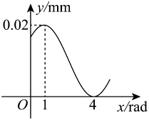
\includegraphics[width=0.2\linewidth]{figure16}
			\caption{}
			\label{fig:figure16}
		\end{figure}

		\begin{enumerate}
			\item[(1)] 求函数 \( f(x) \) 的解析式；
			\item[(2)] 为制造一批特殊钢筋混凝土，现需一批滚道径向残留高度不低于 \(0.015\,\text{mm}\) 且不高于 \(0.02\,\text{mm}\) 的钢筋，若这批钢筋由题中这种 S 型螺纹丝杠旋绕制作，求这种 S 型螺纹丝杠旋绕能制作出符合要求的钢筋的比例。
		\end{enumerate}


		\vspace{3cm}

		\item （15分）

		已知函数 \( g(x) = \dfrac{(x-1)\ln x}{x+1} \)，且函数 \( f(x) \) 的图象与 \( g(x) \) 的图象关于直线 \( x = -1 \) 对称。


		\begin{enumerate}
			\item[(1)] 求 \( f(x) \) 的解析式；
			\item[(2)] 证明：\( f(x) \geq 0 \).
		\end{enumerate}


		\vspace{3cm}

		\item （17分）

		某公司要在一条笔直的道路边安装路灯，要求灯柱 \( AB \) 与地面垂直，灯杆 \( BC \) 与灯柱 \( AB \) 所在的平面与道路走向垂直，路灯 \( C \) 采用锥形灯罩，射出的光线与平面 \( ABC \) 的部分截面如图中阴影部分所示。已知 \(\angle ABC = \dfrac{2}{3}\pi,\ \angle ACD = \dfrac{\pi}{3}\)，路宽 \( AD = 24 \) 米。设 \(\angle BAC = \theta \left( \dfrac{\pi}{12} \leq \theta \leq \dfrac{\pi}{6} \right)\)。

		\begin{figure}[h]
			\centering
			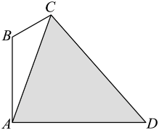
\includegraphics[width=0.2\linewidth]{figure18}
			\caption{}
			\label{fig:figure18}
		\end{figure}

		\begin{enumerate}
			\item[(1)] 若 \(\theta = \dfrac{\pi}{6}\)，求灯柱 \( AB \) 的高 \( h \)；
			\item[(2)] 此公司应该如何设置 \( \theta \) 的值才能使制造路灯灯柱 \( AB \) 与灯杆 \( BC \) 所用材料的总长度最小？最小值为多少？
		\end{enumerate}


		\vspace{3cm}

		\item （17分）

		已知函数 \( f(x) = b - 2a \sin^2 (\omega x + \varphi) \)（\( a > 0,\ \omega > 0,\ |\varphi| < \dfrac{\pi}{2} \)）满足如下条件：

		\begin{enumerate}
			\item[\textcircled{1} ] 函数 \( f(x) \) 的最小值为 \( -3 \)，最大值为 \( 9 \)；
			\item[\textcircled{2} ] \( f\left( \dfrac{1}{2} \right) = 3 \) 且 \( f(1) > 0 \)；
			\item[\textcircled{3} ] 函数 \( f(x) \) 在区间 \([m, n]\) 上是单调函数，且 \( n - m \) 的最大值为 \( 2 \)。
		\end{enumerate}

		试探究并解决如下问题：

		\begin{enumerate}
			\item[(1)] 求 \( \omega \) 的值；
			\item[(2)] 求 \( f(x) \) 在区间 \( \left[ 0, \dfrac{2}{3} \right] \) 上的最小值。
		\end{enumerate}








	\end{enumerate}




\end{document}
